% Created 2021-06-01 Tue 11:25
% Intended LaTeX compiler: pdflatex
\documentclass[presentation, 11pt,  aspectratio=169]{beamer}
\usepackage[utf8]{inputenc}
\usepackage[T1]{fontenc}
\usepackage{graphicx}
\usepackage{grffile}
\usepackage{longtable}
\usepackage{wrapfig}
\usepackage{rotating}
\usepackage[normalem]{ulem}
\usepackage{amsmath}
\usepackage{textcomp}
\usepackage{amssymb}
\usepackage{capt-of}
\usepackage{hyperref}
\usepackage{minted}
\setbeamertemplate{caption}{\raggedright\insertcaption\par}
\usepackage{tcolorbox}
\usepackage{etoolbox}
\BeforeBeginEnvironment{minted}{\begin{tcolorbox}[boxrule=0.5pt}%
\AfterEndEnvironment{minted}{\end{tcolorbox}}%
\usepackage[T1]{fontenc}
\usepackage[utf8]{inputenc}
\definecolor{mydarkred}{RGB}{180, 0, 0}
\renewcommand{\alert}[1]{\textbf{\textcolor{mydarkred}{#1}}}
\hypersetup{colorlinks=false,linkbordercolor={0.2 0.2 0.3},urlbordercolor={0.8 0.8 0.8},pdfborderstyle={/S/U/W 0.5}}
\usetheme{Boadilla}
\usecolortheme{rose}
\author{Giovanni Moretti - giovanni@reflections.co.nz}
\date{\today}
\title{Gemini - a quieter web experience}
\subtitle{niceness through simplicity}
\AtBeginSection{\frame{\sectionpage}}
\hypersetup{
 pdfauthor={Giovanni Moretti - giovanni@reflections.co.nz},
 pdftitle={Gemini - a quieter web experience},
 pdfkeywords={},
 pdfsubject={},
 pdfcreator={Emacs 26.3 (Org mode 9.4.5)}, 
 pdflang={English}}
\begin{document}

\maketitle

\begin{frame}[label={sec:org5e40bdd}]{Problems with WWW}
\begin{itemize}
\item \alert{User tracking}:\\
\begin{itemize}
\item cookies, tracking pixels, browser fingerprinting\\
\end{itemize}

\item \alert{Pages bloated \& source is opaque}\\
\begin{itemize}
\item Google.com: 35 requests - 2.2MB of content - 11 scripts\\
\end{itemize}

\item \alert{Layout \& formatting defined by the creator}\\
\begin{itemize}
\item busy screen -- distracting\\
\item page complexity -- accessibility?\\
\end{itemize}
\pause
\end{itemize}
\vspace{1.5em}
\begin{block}{Web browsers are \emph{really} complicated \ldots{}}
\begin{itemize}
\item HTML-5, CSS-3, JavaScript, rendering images/PDF, playing audio/video, cookies, SSL \ldots{}\\
\item implausible to start from scratch\\
\end{itemize}
\(\rightarrow\) \alert{Attack surface is huge}\\
\end{block}
\end{frame}

\begin{frame}[label={sec:orgd7340ad}]{Gemini}
\begin{block}{Gemini is a new Internet protocol (June 2019)}
\begin{itemize}
\item for distributing of arbitrary files\\
\item lightweight hypertext format\\
\item takes user privacy very seriously\\
\item heavier than Gopher, lighter than the Web, won't replace either\\
\end{itemize}
\pause
\end{block}

\begin{block}{Very different approach to security}
\begin{itemize}
\item very restricted feature set\\
\item whitelist vs. Web's blacklist\\
\end{itemize}
\end{block}
\end{frame}

\begin{frame}[label={sec:org19b3c75}]{Gemini goals}
\begin{block}{Simplicity}
\begin{itemize}
\item a developer can write a client in a weekend\\
\item possible to remember entire protocol spec\\
\begin{itemize}
\item \(\approx\)600 lines (12 x A4 pages)\\
\end{itemize}
\end{itemize}
\end{block}

\begin{block}{It will be \emph{difficult to extend} in the future}
so it \alert{stays} simple and privacy conscious\\
\end{block}

\begin{block}{Gemini's designer intended:}
\begin{itemize}
\item one request, one response: no hidden network activity\\
\item images can be inlined OR loaded in external viewer -- \alert{client decides}\\
\end{itemize}
\end{block}
\end{frame}


\begin{frame}[label={sec:orgce98e5f}]{Why not use a subset of HTML?}
\begin{itemize}
\item there'd be no clear separation between Gemini and HTML sites\\
\item browser would still interpret whatever was sent - you never know\\
\begin{itemize}
\item request page of text \(\rightarrow\) browser loads hidden iframes and 15 scripts \ldots{}\\
\end{itemize}
\item too tempting to 'add just one more feature'\\
\item tracking/user profiling would still work\\
\end{itemize}
\end{frame}


\begin{frame}[label={sec:org688e6a6}]{Gemini - Text formatting}
\begin{itemize}
\item UTF-8 is the default\\
\item no inline formatting: i.e. no bold/italics\\
\item all text except preformatted blocks are line-wrapped\\
\item \alert{ALL} styling is done by the client\\
\end{itemize}
\end{frame}


\begin{frame}[label={sec:org595aef2}]{Gemini Markup is line-oriented}
\begin{block}{Six core elements}
\begin{center}
\begin{tabular}{ll}
 & \\
Line Type & Start of line\\
\hline
\alert{Heading} & \# ~ \#\# ~ \#\#\#\\
\alert{List item} & *\\
\alert{Quote} & >\\
\alert{Preformatted text} & \alert{```} line before and after\\
\alert{Link} & =>\\
\alert{Body Text} & all else\\
\hline
link examples & => \href{gemini://gemini.circumlunar.space}{gemini://gemini.circumlunar.space}\\
 & => \url{https://www.reddit.com} REDDIT Home Page\\
 & => image-dir/giant-peach.jpg\\
 & => \url{mailto:fred@example.com}  Email me\\
 & => \href{gemini://podcast.com/episode-1.mp3}{gemini://podcast.com/episode-1.mp3}\\
\hline
\end{tabular}
\end{center}
\end{block}
\end{frame}


\begin{frame}[label={sec:org714b87a},fragile]{Sample Gemini page - \href{gemini://friendo.monster/log/lace.gmi}{gemini://friendo.monster/log/lace.gmi} - 3314 bytes}
 \begin{scriptsize}
\begin{verbatim}
# A script to interleave tiny Gemini logs
18 Feb 2021

I guess what this script is, really, is a client-of-sorts for Gemini tiny logs. Which is kinda like micro-blogging on Gemini.

*Client* is overstating it though. It's written in the laziest, simplest way I can think of and it will collapse if the content is not as it expects.

Let's call it a first pass.

=> https://gitlab.com/uoou/dotfiles/-/tree/master/stow/bin/home/drew/.local/bin/lace

If you want to give it a go, just

```
wget https://gitlab.com/uoou/dotfiles/-/raw/master/stow/bin/home/drew/.local/bin/lace
chmod +x lace
```

And then either put it somewhere in your `$PATH` or call it with `./lace`.

Here's what it looks like *in action*...

=> /images/lace.png

## How do it works?

To add a subscription to a tiny log, just do
\end{verbatim}
\end{scriptsize}
\end{frame}

\begin{frame}[label={sec:org5afd7ce}]{Rendered in Lagrange}
\begin{center}
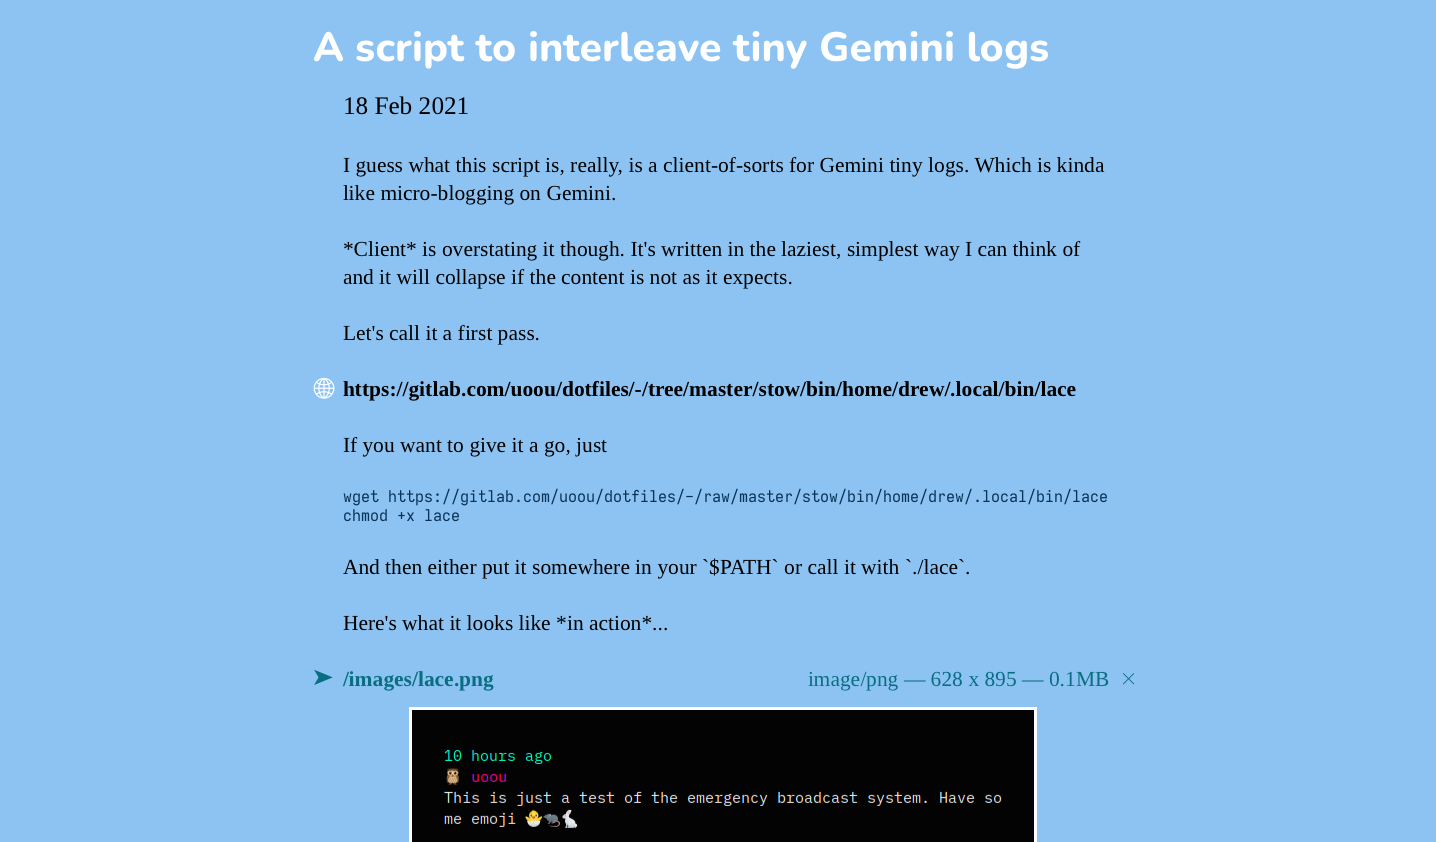
\includegraphics[width=.9\linewidth]{images/gemini-sample-friendo.monster.png}
\end{center}
\end{frame}

\begin{frame}[label={sec:org3cc578a}]{or with a dark theme}
\begin{center}
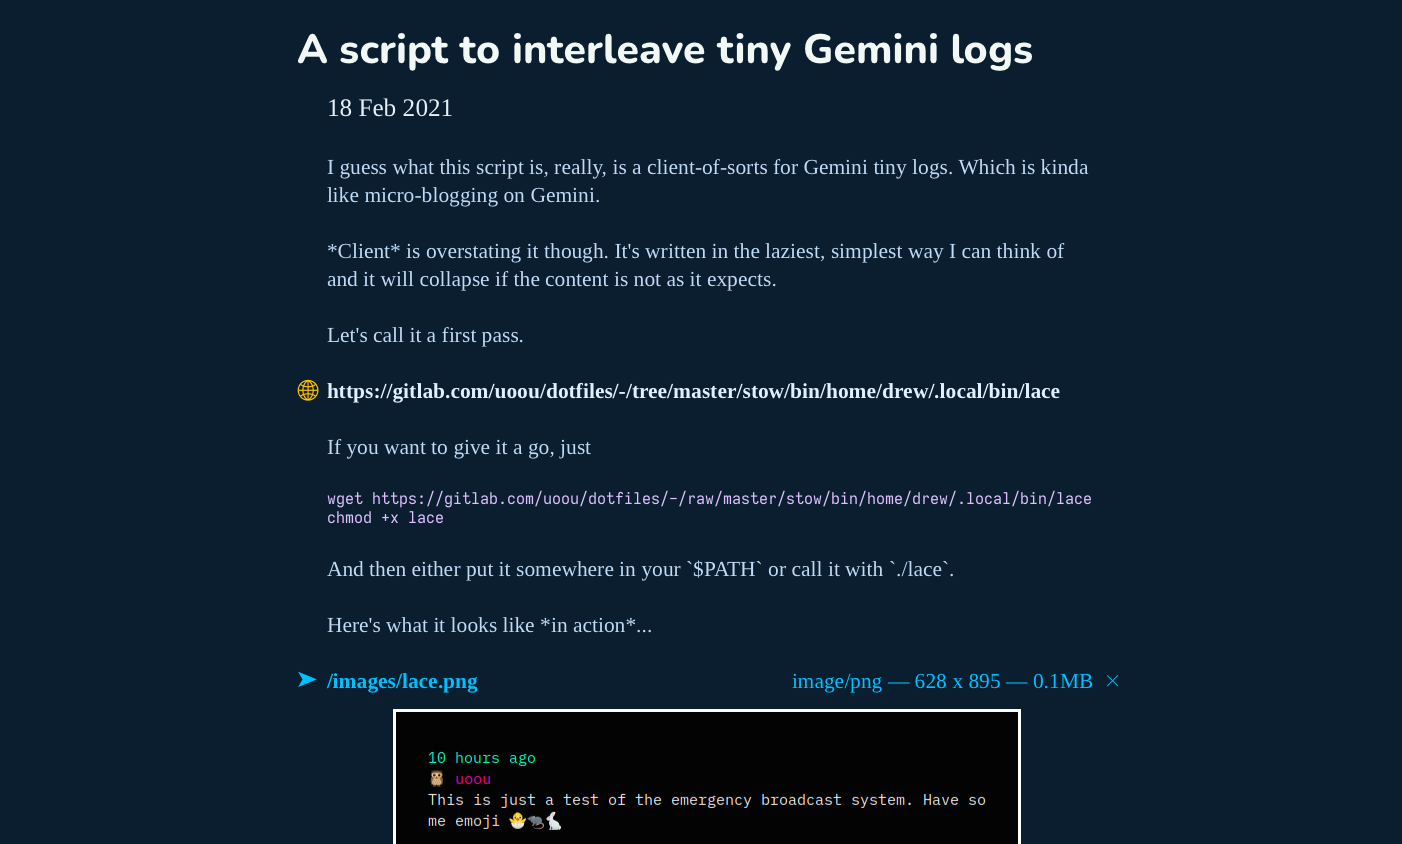
\includegraphics[width=.9\linewidth]{images/gemini-sample-lace-dark.png}
\end{center}
\end{frame}
\begin{frame}[label={sec:org81e0c5c}]{Gemini clients control the page style}
\begin{figure}[htbp]
\centering
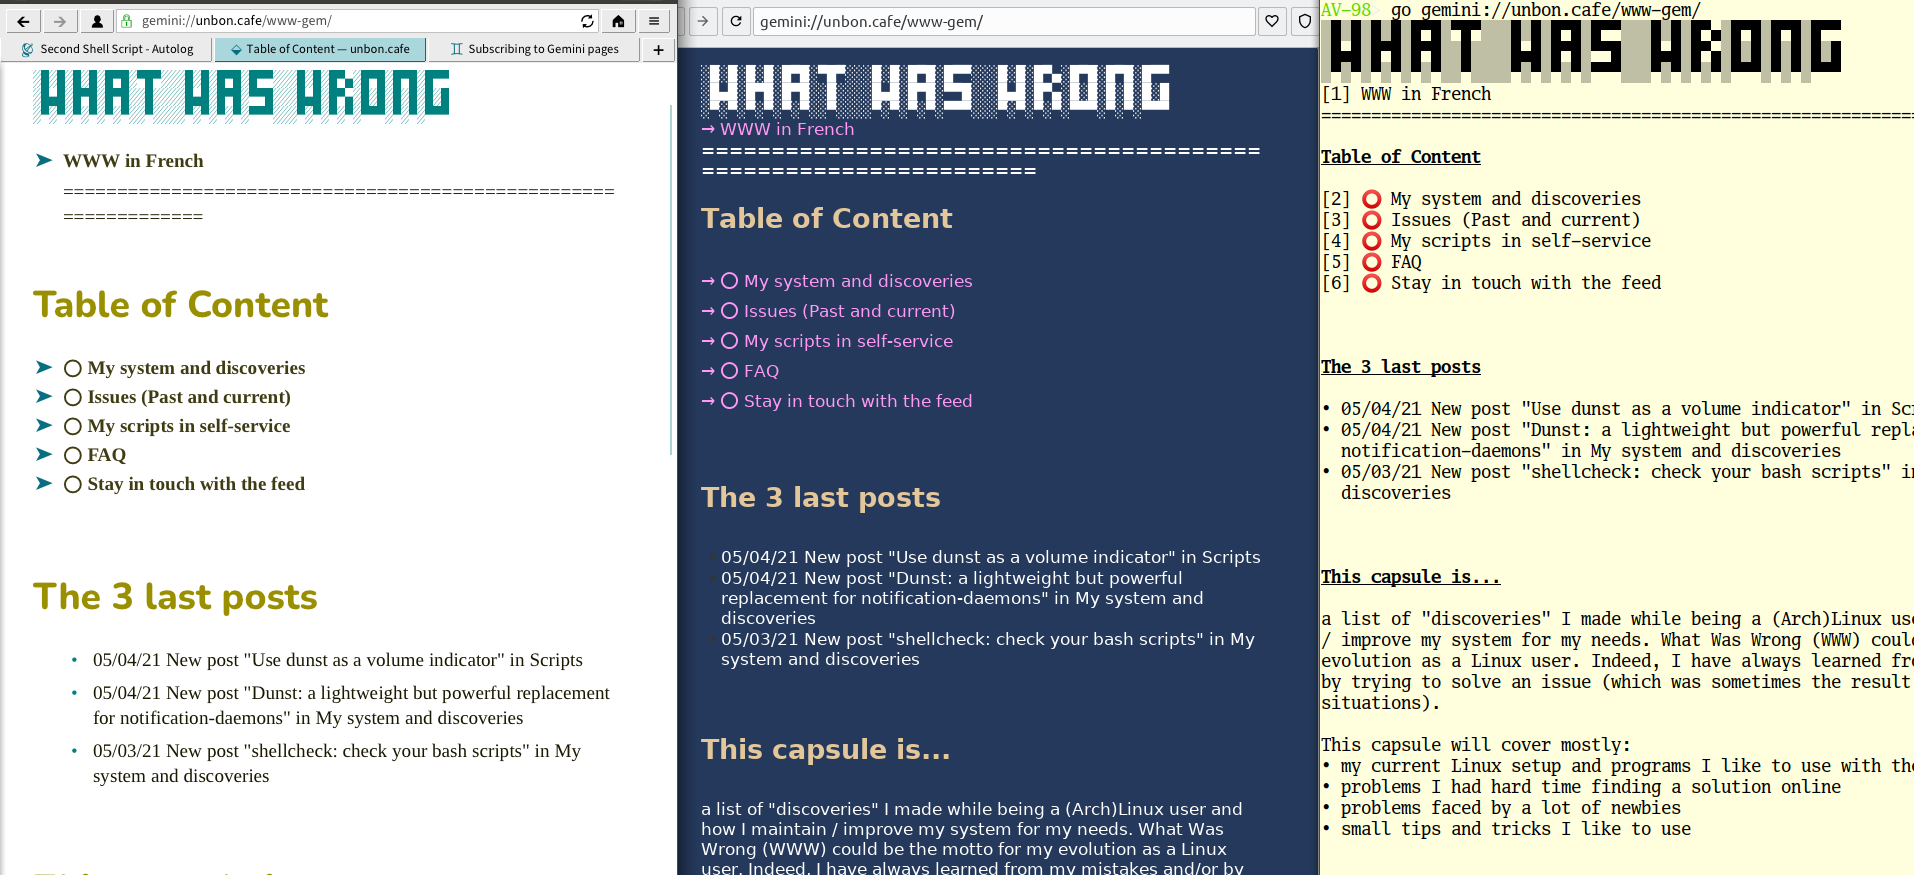
\includegraphics[width=0.95\textwidth]{images/threebrowsers.png}
\caption{Same page - three browsers: Lagrange, Kristall and AV98 (terminal)}
\end{figure}
\end{frame}

\begin{frame}[label={sec:orgd8f222e}]{Let's see what Gemini users have created}
\begin{center}
\begin{tabular}{c}
Demo:   selection of Gemini pages viewed in Lagrange\\
\\
\end{tabular}
\end{center}
\end{frame}

\begin{frame}[label={sec:orgae5e22b}]{What's the protocol: Gemini Request/Response}
\begin{quote}
\begin{enumerate}
\item Client: Opens connection\\
\item Server: Accepts connection\\
\item Client/Server: Complete TLS handshake\\
\item Client: Validates server certificate\\
\item \alert{Client: Sends one line Request-URL or URL+query-string}\\
\item \alert{Server: Sends one line response header}\\
\item \alert{Server: Sends response body (text/binary data)}, Closes connection\\
\item \alert{Client: Handles response}\\
\end{enumerate}
\end{quote}
\end{frame}

\begin{frame}[label={sec:orgd7e7b0b}]{Using TLS Certificates}
\begin{block}{Gemini uses TLS v1.3 (ideally) or v1.2}
\begin{itemize}
\item no certificate authority required\\
\item users are based on "Trust on First Use" (TOFU) - like SSH\\
\end{itemize}

\pause
\end{block}
\begin{block}{No Cookies: identify users by their TLS certificate}
\begin{itemize}
\item clients support multiple certificates - user chooses\\
\item if a certificate is deleted, that identity is \emph{gone}\\
\end{itemize}
\end{block}
\end{frame}


\begin{frame}[label={sec:orgc35ad1d}]{Gemini Software}
\begin{block}{Desktop browsers}
\begin{itemize}
\item \alert{Lagrange} - \url{https://github.com/skyjake/lagrange/releases/tag/v1.4.0}\\
\item \alert{Kristall} - \url{https://github.com/MasterQ32/kristall}\\
\item \alert{Amfora \& AV98} - terminal based clients\\
\item \alert{Elpher} for Emacs - via Melpa\\
\end{itemize}
\end{block}
\begin{block}{Mobile browsers}
\begin{itemize}
\item \alert{Android} - Ariane from Play Store \alert{\(\leftarrow\) Easy to try}\\
\item \alert{iPhone/Pad} - Elaho from App Store and \url{https://github.com/pitr/gemini-ios}\\
\end{itemize}
\end{block}

\begin{block}{Recommended Servers: Agate (Rust) \& Jetforce (Python)}
There's \emph{lots} of gemini software: \url{https://gemini.circumlunar.space/software/}\\
\end{block}
\end{frame}
\begin{frame}[label={sec:org6188524}]{Quick overview of Lagrange}
\emph{Lagrange} - the most feature-rich Gemini browser:\\
\begin{itemize}
\item it looks really nice!\\
\item multiple tabs\\
\item subscriptions\\
\item inlining of images and audio\\
\item clear certificate management\\
\item split-screen view\\
\item available for Linux, Mac and Windows\\
\end{itemize}
\end{frame}


\begin{frame}[label={sec:org02d3bba}]{Subscribing to Gemini pages}
Options: Browser detects change in page headings OR simple day-timestamp scheme:\\
\begin{footnotesize}
\begin{quote}
Welcome to my Gemlog, where you can read every Friday about my adventures in urban gardening and abstract algebra!\\

\#\# My posts\\
=> \alert{bokashi.gmi              2020-11-20 - Early Bokashi composting experiments}\\
=> \alert{finite-simple-groups.gmi 2020-11-13 - Trying to get to grips with finite simple groups\ldots{}}\\
=> \alert{balcony.gmi              2020-11-06 - I started a balcony garden!}\\

\#\# Other gemlogs I enjoy\\
=> \href{gemini://example.com/foo/}{gemini://example.com/foo/}    Abelard Lindsay's gemlog\\
=> \href{gemini://example.net/bar/}{gemini://example.net/bar/}    Vladimir Harkonnen's gemlog\\
=> \href{gemini://example.org/baz/}{gemini://example.org/baz/}    Case Pollard's gemlog\\
\end{quote}
\end{footnotesize}
from \href{gemini://gemini.circumlunar.space/docs/companion/subscription.gmi}{gemini://gemini.circumlunar.space/docs/companion/subscription.gmi}\\
\end{frame}

\begin{frame}[label={sec:orgc8ec4fe}]{What are people doing with it?}
\begin{itemize}
\item \alert{Blogging} -- \href{gemini://fixato.org/2020-03-25-an-uneventful-day.gmi}{gemini://fixato.org/2020-03-25-an-uneventful-day.gmi}\\
\item \alert{Podcasts} -- \href{gemini://gem.chriswere.uk/trendytalk/}{gemini://gem.chriswere.uk/trendytalk/}\\
\item \alert{News sites proxied to Gemini:} \href{gemini://simplynews.metalune.xyz}{gemini://simplynews.metalune.xyz}\\
\item \alert{Gembooks - an eBook format using Gemini:}\\
\begin{itemize}
\item \url{https://codeberg.org/oppenlab/gempub}\\
\end{itemize}
\item \alert{Blogging Client in 30 lines} \\
-- \href{gemini://spool-five.com/gemlog/2021-04-01-second_script.gmi}{gemini://spool-five.com/gemlog/2021-04-01-second_script.gmi}\\
\item \alert{xj9 - tech blog} \href{gemini://sunshinegardens.org/~xj9}{gemini://sunshinegardens.org/~xj9}\\
\item \alert{Sunshine Gardens:} \href{gemini://sunshinegardens.org}{gemini://sunshinegardens.org}\\
\item \alert{One Hundred Rabbits (resilience, offline-first, sailing, cooking, Plan9, design):}$\backslash$\ \href{gemini://gemini.circumlunar.space/users/hundredrabbits}{gemini://gemini.circumlunar.space/users/hundredrabbits}\\
\item \alert{Konpeito is quarterly Lo-fi hip-hop \& chill mixtape} - \href{gemini://konpeito.media}{gemini://konpeito.media}\\
\end{itemize}

On Social Media: Mastodon - \url{https://mastodon.social/tags/gemini}\\
\end{frame}


\begin{frame}[label={sec:org323b731}]{Small Web (smolweb) related sites}
\begin{itemize}
\item \alert{Tilde sites:} e.g.\\
\begin{itemize}
\item \url{https://tildeverse.org/} \\
\item \url{https://tilde.team/} \\
\item \href{gemini://tilde.team}{gemini://tilde.team}  -- Free Gemini Hosting\\
\end{itemize}
\item \alert{Pubnixes:} Public Unix servers\\
Super Dimensional Fortress:\\
\begin{itemize}
\item \url{https://sdf.org}\\
\item \url{https://sdfeu.org}\\
\end{itemize}
\end{itemize}
\end{frame}


\begin{frame}[label={sec:org46722ee}]{Konpeito Retro tapes - announced on Mastodon.social}
\begin{figure}[htbp]
\centering
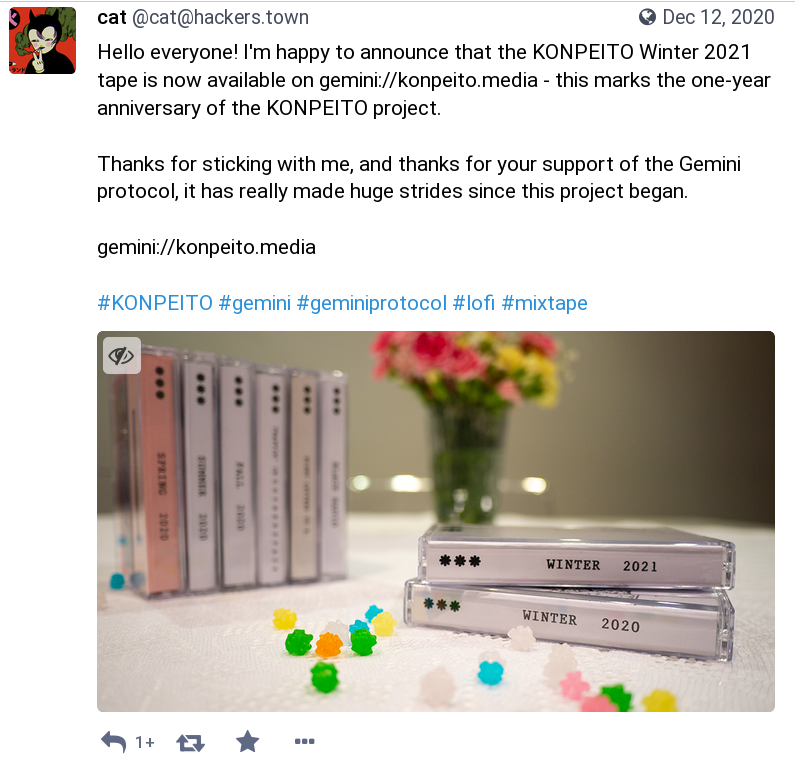
\includegraphics[height=0.75\textheight]{images/konpeito-1.png}
\caption{\href{gemini://konpeito.media}{gemini://konpeito.media}}
\end{figure}
\end{frame}

\begin{frame}[label={sec:org75e4aab}]{Konpeito inside Lagrange browser - expanded view}
\begin{center}
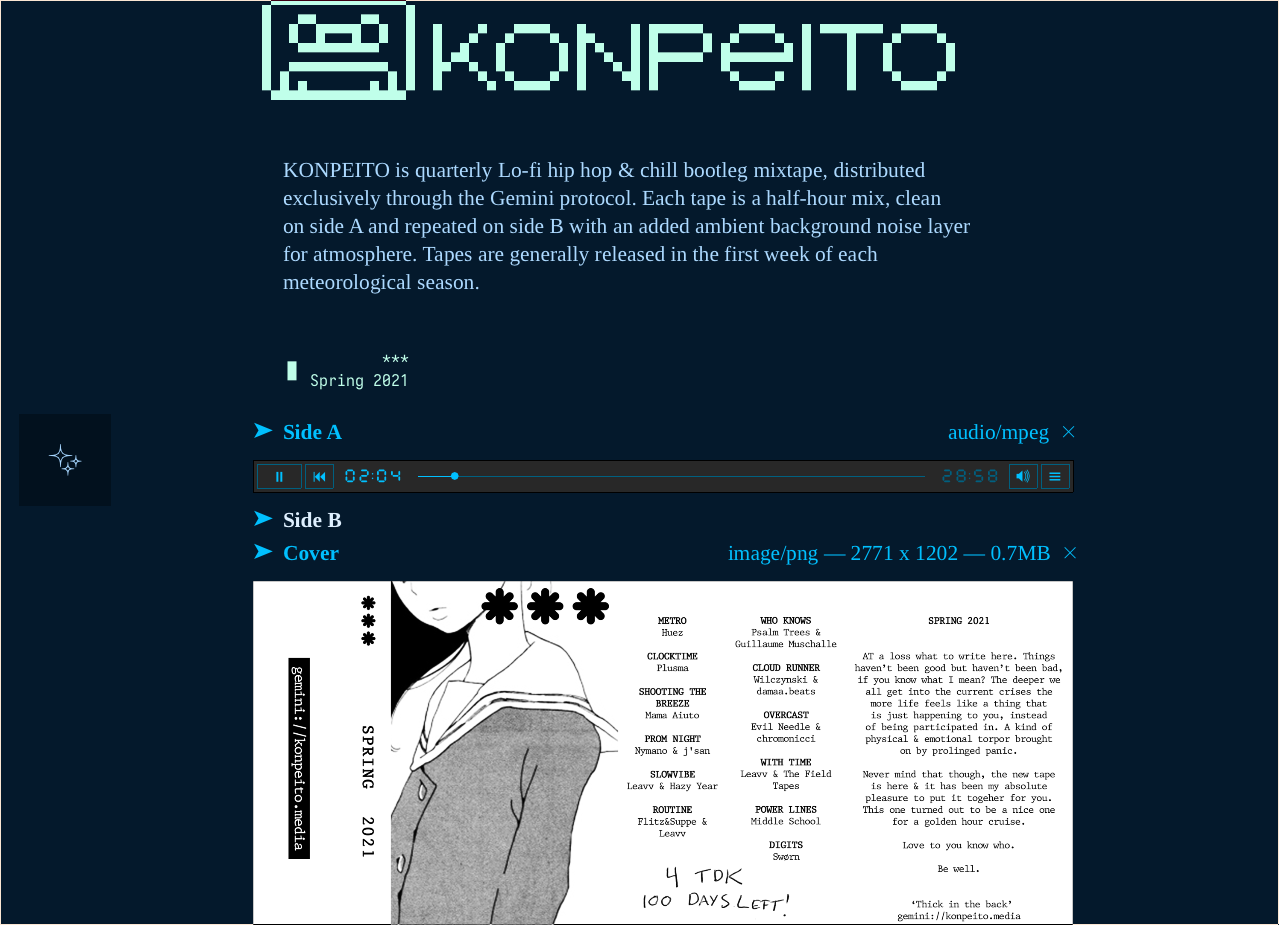
\includegraphics[width=0.75\linewidth]{images/konpeito-expanded-in-Lagrange.png}
\end{center}
\end{frame}

\begin{frame}[label={sec:org2261133}]{Why do you like Gemini?}
\vspace{2em}
\begin{quote}
@pytpu it just works. No cookies/tracking/ads or broken web standards.\\

It's simply your content presented in the way you want it to be. \ldots\\

Also all the people around there are nice and friendly \ldots{}\\

\alert{This shouldn't just co-exist with the web, \\
it should be default for everyone.}\\

\begin{scriptsize}
Leonie <@koyu@koyu.space> -- \url{https://koyu.space/@koyu/106113153639591891}\\
\end{scriptsize}
\end{quote}

\vspace{2em}
\begin{scriptsize}
Survey summary: \href{gemini://nytpu.com/why-gemini.gmi}{gemini://nytpu.com/why-gemini.gmi}\\
\end{scriptsize}
\end{frame}


\begin{frame}[label={sec:orge1ad6cc}]{Conclusion}
\begin{block}{Gemini}
\begin{itemize}
\item \alert{for users}\\
\begin{itemize}
\item a very simple and accessible markup for creating pages\\
\item suitable for many (but not all) documents\\
\item provides an ad-free, secure, and distraction-free environment\\
\end{itemize}

\item \alert{for developers}\\
\begin{itemize}
\item is simple enough to encourage experimentation\\
\item gemtext markup is easily mapped to other formats\\
\item has low hardware and network traffic requirements\\
\end{itemize}
\end{itemize}
\pause
\end{block}
\begin{block}{Interested?}
\begin{itemize}
\item \alert{Getting Started with Gemini:} \href{gemini://geminiquickst.art}{gemini://geminiquickst.art} \(\leftarrow\) \alert{Really Good}\\
\item \alert{Gemini Home:} \url{https://gemini.circumlunar.space}\\
\item \alert{Gemini on Mastodon:} \url{https://mastodon.social/web/timelines/tag/gemini}\\
\end{itemize}
\end{block}
\end{frame}


\begin{frame}[label={sec:org8fc7fc5}]{Reuse/License}
\begin{block}{Reuse this presentation}
\begin{center}

\includegraphics[width=0.25\textwidth]{images-external/cc-by-sa.png}
\end{center}

\begin{small}
This presentation is Copyright (C) 2021 Giovanni Moretti.\\

This work is licensed under a Creative Commons Attribution-ShareAlike 4.0 International License. For more information, go to\\
~~ \url{http://creativecommons.org/licenses/by-sa/4.0/}\\
\end{small}
\end{block}
\end{frame}
\end{document}